% Options for packages loaded elsewhere
\PassOptionsToPackage{unicode}{hyperref}
\PassOptionsToPackage{hyphens}{url}
%
\documentclass[
]{article}
\usepackage{lmodern}
\usepackage{amssymb,amsmath}
\usepackage{ifxetex,ifluatex}
\ifnum 0\ifxetex 1\fi\ifluatex 1\fi=0 % if pdftex
  \usepackage[T1]{fontenc}
  \usepackage[utf8]{inputenc}
  \usepackage{textcomp} % provide euro and other symbols
\else % if luatex or xetex
  \usepackage{unicode-math}
  \defaultfontfeatures{Scale=MatchLowercase}
  \defaultfontfeatures[\rmfamily]{Ligatures=TeX,Scale=1}
\fi
% Use upquote if available, for straight quotes in verbatim environments
\IfFileExists{upquote.sty}{\usepackage{upquote}}{}
\IfFileExists{microtype.sty}{% use microtype if available
  \usepackage[]{microtype}
  \UseMicrotypeSet[protrusion]{basicmath} % disable protrusion for tt fonts
}{}
\makeatletter
\@ifundefined{KOMAClassName}{% if non-KOMA class
  \IfFileExists{parskip.sty}{%
    \usepackage{parskip}
  }{% else
    \setlength{\parindent}{0pt}
    \setlength{\parskip}{6pt plus 2pt minus 1pt}}
}{% if KOMA class
  \KOMAoptions{parskip=half}}
\makeatother
\usepackage{xcolor}
\IfFileExists{xurl.sty}{\usepackage{xurl}}{} % add URL line breaks if available
\IfFileExists{bookmark.sty}{\usepackage{bookmark}}{\usepackage{hyperref}}
\hypersetup{
  pdftitle={A Study on Alcohol Intake and Longevity},
  pdfauthor={Shouyang Wang\^{}\{1\}, Drake Wastson\^{}\{2\}},
  hidelinks,
  pdfcreator={LaTeX via pandoc}}
\urlstyle{same} % disable monospaced font for URLs
\usepackage[margin=1in]{geometry}
\usepackage{color}
\usepackage{fancyvrb}
\newcommand{\VerbBar}{|}
\newcommand{\VERB}{\Verb[commandchars=\\\{\}]}
\DefineVerbatimEnvironment{Highlighting}{Verbatim}{commandchars=\\\{\}}
% Add ',fontsize=\small' for more characters per line
\usepackage{framed}
\definecolor{shadecolor}{RGB}{255,255,255}
\newenvironment{Shaded}{\begin{snugshade}}{\end{snugshade}}
\newcommand{\AlertTok}[1]{\textcolor[rgb]{0.75,0.01,0.01}{\textbf{\colorbox[rgb]{0.97,0.90,0.90}{#1}}}}
\newcommand{\AnnotationTok}[1]{\textcolor[rgb]{0.79,0.38,0.79}{#1}}
\newcommand{\AttributeTok}[1]{\textcolor[rgb]{0.00,0.34,0.68}{#1}}
\newcommand{\BaseNTok}[1]{\textcolor[rgb]{0.69,0.50,0.00}{#1}}
\newcommand{\BuiltInTok}[1]{\textcolor[rgb]{0.39,0.29,0.61}{\textbf{#1}}}
\newcommand{\CharTok}[1]{\textcolor[rgb]{0.57,0.30,0.62}{#1}}
\newcommand{\CommentTok}[1]{\textcolor[rgb]{0.54,0.53,0.53}{#1}}
\newcommand{\CommentVarTok}[1]{\textcolor[rgb]{0.00,0.58,1.00}{#1}}
\newcommand{\ConstantTok}[1]{\textcolor[rgb]{0.67,0.33,0.00}{#1}}
\newcommand{\ControlFlowTok}[1]{\textcolor[rgb]{0.12,0.11,0.11}{\textbf{#1}}}
\newcommand{\DataTypeTok}[1]{\textcolor[rgb]{0.00,0.34,0.68}{#1}}
\newcommand{\DecValTok}[1]{\textcolor[rgb]{0.69,0.50,0.00}{#1}}
\newcommand{\DocumentationTok}[1]{\textcolor[rgb]{0.38,0.47,0.50}{#1}}
\newcommand{\ErrorTok}[1]{\textcolor[rgb]{0.75,0.01,0.01}{\underline{#1}}}
\newcommand{\ExtensionTok}[1]{\textcolor[rgb]{0.00,0.58,1.00}{\textbf{#1}}}
\newcommand{\FloatTok}[1]{\textcolor[rgb]{0.69,0.50,0.00}{#1}}
\newcommand{\FunctionTok}[1]{\textcolor[rgb]{0.39,0.29,0.61}{#1}}
\newcommand{\ImportTok}[1]{\textcolor[rgb]{1.00,0.33,0.00}{#1}}
\newcommand{\InformationTok}[1]{\textcolor[rgb]{0.69,0.50,0.00}{#1}}
\newcommand{\KeywordTok}[1]{\textcolor[rgb]{0.12,0.11,0.11}{\textbf{#1}}}
\newcommand{\NormalTok}[1]{\textcolor[rgb]{0.12,0.11,0.11}{#1}}
\newcommand{\OperatorTok}[1]{\textcolor[rgb]{0.12,0.11,0.11}{#1}}
\newcommand{\OtherTok}[1]{\textcolor[rgb]{0.00,0.43,0.16}{#1}}
\newcommand{\PreprocessorTok}[1]{\textcolor[rgb]{0.00,0.43,0.16}{#1}}
\newcommand{\RegionMarkerTok}[1]{\textcolor[rgb]{0.00,0.34,0.68}{\colorbox[rgb]{0.88,0.91,0.97}{#1}}}
\newcommand{\SpecialCharTok}[1]{\textcolor[rgb]{0.24,0.68,0.91}{#1}}
\newcommand{\SpecialStringTok}[1]{\textcolor[rgb]{1.00,0.33,0.00}{#1}}
\newcommand{\StringTok}[1]{\textcolor[rgb]{0.75,0.01,0.01}{#1}}
\newcommand{\VariableTok}[1]{\textcolor[rgb]{0.00,0.34,0.68}{#1}}
\newcommand{\VerbatimStringTok}[1]{\textcolor[rgb]{0.75,0.01,0.01}{#1}}
\newcommand{\WarningTok}[1]{\textcolor[rgb]{0.75,0.01,0.01}{#1}}
\usepackage{longtable,booktabs}
% Correct order of tables after \paragraph or \subparagraph
\usepackage{etoolbox}
\makeatletter
\patchcmd\longtable{\par}{\if@noskipsec\mbox{}\fi\par}{}{}
\makeatother
% Allow footnotes in longtable head/foot
\IfFileExists{footnotehyper.sty}{\usepackage{footnotehyper}}{\usepackage{footnote}}
\makesavenoteenv{longtable}
\usepackage{graphicx,grffile}
\makeatletter
\def\maxwidth{\ifdim\Gin@nat@width>\linewidth\linewidth\else\Gin@nat@width\fi}
\def\maxheight{\ifdim\Gin@nat@height>\textheight\textheight\else\Gin@nat@height\fi}
\makeatother
% Scale images if necessary, so that they will not overflow the page
% margins by default, and it is still possible to overwrite the defaults
% using explicit options in \includegraphics[width, height, ...]{}
\setkeys{Gin}{width=\maxwidth,height=\maxheight,keepaspectratio}
% Set default figure placement to htbp
\makeatletter
\def\fps@figure{htbp}
\makeatother
\setlength{\emergencystretch}{3em} % prevent overfull lines
\providecommand{\tightlist}{%
  \setlength{\itemsep}{0pt}\setlength{\parskip}{0pt}}
\setcounter{secnumdepth}{-\maxdimen} % remove section numbering

\title{\textbf{A Study on Alcohol Intake and Longevity}}
\usepackage{etoolbox}
\makeatletter
\providecommand{\subtitle}[1]{% add subtitle to \maketitle
  \apptocmd{\@title}{\par {\large #1 \par}}{}{}
}
\makeatother
\subtitle{\emph{Is Alcohol Consumption Linked to Longer Lifespan?}}
\author{Shouyang Wang\(^{1}\), Drake Wastson\(^{2}\)}
\date{}

\begin{document}
\maketitle

\begin{center}
$^{1}$ UW Information School, wang20@uw.edu

$^{2}$ University of Washington, drakerw@uw.edu
\end{center}

\hypertarget{introduction}{%
\subsection{Introduction}\label{introduction}}

Researchers have extensively studied the relationship between alcohol
consumption and longevity. However, it is a common phenomenon that the
findings obtained by one author differ from the result of others on such
topics due to a difference in research methodology and data collection.
On the one hand, studies suggest ``drinking about two glasses of wine or
beer a day was linked to an 18\% drop in person's risk of early
death.''\footnote{Jamie Ducharme, ``Can Alcohol Help You Live Longer?
  Here's What the Research Really Says,'' Time, February 20, 2018,
  \url{https://time.com/5166514/moderate-drinking-live-longer-study/}.}
On the other hand, some researchers challenge the findings by stating
that ``the more alcohol a person drinks, the higher their risk of early
death.''\footnote{Angela Wood and Ellie Paige, ``Drinking a Pint of Beer
  May Lower Your Life Expectancy by the Same Amount as Smoking a
  Cigarette -- New Research,'' The Conversation, April 12, 2018,
  \url{https://theconversation.com/drinking-a-pint-of-beer-may-lower-your-life-expectancy-by-the-same-amount-as-smoking-a-cigarette-new-research-90346}.}
What, then, is the truth? Could it also be possible that there is no
relationship between the two entities?

This project will make use of three separate data sets from the
\emph{World Bank} data repository in order to answer the following
question: \textbf{Does alcohol consumption lead to longer life
expectancy?} In order to address this question, we will use
international country-level data that quantifies alcohol consumption,
average life expectancy, and also GDP (to address a possible
confounder). Alcohol consumption is a virtually universal trait among
cultures across the world and is an aspect of human life that may be
playing a part in determining the length of our collective life spans.
From time to time there will be popular scientific articles detailing
the health benefits of a nightly glass of wine or another article
arguing the contrary, so it would be insightful to see if there is any
support for either side of the argument provided by demographic data on
an international scale.

For this study, our null hypothesis will be that alcohol consumption has
\emph{no relationship} with the life expectancy per capita, and the
alternative hypothesis that we are interested in exploring is that
alcohol consumption \emph{is linked} to longevity. If there is a
relationship, we can then explore if the relationship is positive or
negative.

\begin{quote}
\(H_{o}\): alcohol consumption is not linked to life expectancy

\(H_{a}\): alcohol consumption is linked to life expectancy

\(\alpha: 0.05\)
\end{quote}

\begin{center}\rule{0.5\linewidth}{0.5pt}\end{center}

\hypertarget{data}{%
\subsection{Data}\label{data}}

As stated in the introduction, the source of our data will be the
\emph{World Bank}, which is an online repository of national and
international statistics put together by the \emph{World Bank's
Development Data Group}. The majority of these statistics are provided
by the statistical systems of the countries themselves. The \emph{World
Bank} also works to assist underdeveloped countries with the
implementation of statistical systems and attempts to raise awareness of
the importance of data driven decision making. This report will make use
of 3 specific data sets which are detailed below:

\begin{itemize}
\item
  \textbf{GDP(\$):} Measured by GDP per capita by current international
  currency rates. Link:
  \url{https://data.worldbank.org/indicator/NY.GDP.PCAP.PP.CD}
\item
  \textbf{Life Expectancy(Years):} Measured by average life expectancy
  at birth in years. Link:
  \url{https://data.worldbank.org/indicator/SP.DYN.LE00.IN}
\item
  \textbf{Alcohol Consumption(Liters):} Measured in alcohol consumption
  per capita by liter of pure alcohol. Link:
  \url{https://data.worldbank.org/indicator/SH.ALC.PCAP.LI}
\end{itemize}

\begin{Shaded}
\begin{Highlighting}[]
\NormalTok{gdp_df <-}\StringTok{ }\KeywordTok{read.csv}\NormalTok{(}\StringTok{"data/gdp.csv"}\NormalTok{, }
                   \DataTypeTok{fileEncoding=}\StringTok{"UTF-8-BOM"}\NormalTok{,}
                   \DataTypeTok{stringsAsFactors =} \OtherTok{FALSE}\NormalTok{) }\OperatorTok\StringTok{ }
\StringTok{          }\KeywordTok{select}\NormalTok{(name, Country.Code, X2018) }\OperatorTok\StringTok{ }
\StringTok{          }\KeywordTok{rename}\NormalTok{(}\DataTypeTok{GDP =}\NormalTok{ X2018)}

\NormalTok{life_exp_df <-}\StringTok{ }\KeywordTok{read.csv}\NormalTok{(}\StringTok{"data/life_exp.csv"}\NormalTok{,}
                        \DataTypeTok{fileEncoding=}\StringTok{"UTF-8-BOM"}\NormalTok{,}
                        \DataTypeTok{stringsAsFactors =} \OtherTok{FALSE}\NormalTok{) }\OperatorTok\StringTok{ }
\StringTok{                }\KeywordTok{select}\NormalTok{(name, Country.Code, X2018) }\OperatorTok\StringTok{ }
\StringTok{                }\KeywordTok{rename}\NormalTok{(}\DataTypeTok{life_exp =}\NormalTok{ X2018)}

\NormalTok{alcohol_df <-}\StringTok{ }\KeywordTok{read.csv}\NormalTok{(}\StringTok{"data/alcohol.csv"}\NormalTok{, }
                       \DataTypeTok{fileEncoding=}\StringTok{"UTF-8-BOM"}\NormalTok{,}
                       \DataTypeTok{stringsAsFactors =} \OtherTok{FALSE}\NormalTok{) }\OperatorTok\StringTok{ }
\StringTok{              }\KeywordTok{select}\NormalTok{(name, Country.Code, X2018) }\OperatorTok\StringTok{ }
\StringTok{              }\KeywordTok{rename}\NormalTok{(}\DataTypeTok{alcohol_consum =}\NormalTok{ X2018)}
\end{Highlighting}
\end{Shaded}

\hypertarget{limitations-of-the-datasetstudy}{%
\subsection{Limitations of the
Dataset/Study}\label{limitations-of-the-datasetstudy}}

The World Bank Open Data is recognized as a valid data source globally.
However, there is no such thing as a perfect data set. The way that the
data is collected and the quality of the information is crucial to yield
the most accurate results possible that resemble reality.

\hypertarget{null-values}{%
\subsubsection{Null Values}\label{null-values}}

The section aims to scrutinize the null/missing values in the data set

\begin{Shaded}
\begin{Highlighting}[]
\CommentTok{#merge all three datasets }
\NormalTok{temp_merge <-}\StringTok{ }\NormalTok{gdp_df }\OperatorTok\StringTok{ }\KeywordTok{inner_join}\NormalTok{(alcohol_df) }\OperatorTok\StringTok{ }\KeywordTok{inner_join}\NormalTok{(life_exp_df)}

\KeywordTok{colSums}\NormalTok{(}\KeywordTok{is.na}\NormalTok{(temp_merge)) }\OperatorTok\StringTok{ }
\StringTok{  }\KeywordTok{as.data.frame}\NormalTok{() }\OperatorTok\StringTok{ }
\StringTok{  }\KeywordTok{mutate}\NormalTok{(}\DataTypeTok{prop =} \KeywordTok{paste0}\NormalTok{(}\KeywordTok{round}\NormalTok{(. }\OperatorTok{*}\StringTok{ }\DecValTok{100} \OperatorTok{/}\StringTok{ }\KeywordTok{nrow}\NormalTok{(temp_merge), }\DecValTok{2}\NormalTok{), }\StringTok{"%"}\NormalTok{)) }\OperatorTok\StringTok{ }
\StringTok{           }\KeywordTok{kable}\NormalTok{(}\DataTypeTok{caption =} \StringTok{"Null Count & Null Proportion in World Bank Data"}\NormalTok{,}
                 \DataTypeTok{col.names =} \KeywordTok{c}\NormalTok{(}\StringTok{"count"}\NormalTok{, }\StringTok{"proportion"}\NormalTok{), }\DataTypeTok{alight =} \StringTok{"r"}\NormalTok{)}
\end{Highlighting}
\end{Shaded}

\begin{longtable}[]{@{}lrl@{}}
\caption{Null Count \& Null Proportion in World Bank
Data}\tabularnewline
\toprule
& count & proportion\tabularnewline
\midrule
\endfirsthead
\toprule
& count & proportion\tabularnewline
\midrule
\endhead
name & 0 & 0\%\tabularnewline
Country.Code & 0 & 0\%\tabularnewline
GDP & 25 & 9.51\%\tabularnewline
alcohol\_consum & 31 & 11.79\%\tabularnewline
life\_exp & 20 & 7.6\%\tabularnewline
\bottomrule
\end{longtable}

The analysis suggests we have roughly 10\% missing data. Missing data
has a significant impact when calculating the outcome variable based on
inferential statistics.

\hypertarget{time-matters}{%
\subsubsection{Time Matters}\label{time-matters}}

We used the data collected from 2018. The intuition is that 2018 is the
most recent year in the World Bank data set with the most comprehensive
information on all three entities of interest. It is unclear if the
findings reflect the current situation.

\hypertarget{alcohol-consumption-per-capita}{%
\subsubsection{Alcohol Consumption Per
Capita}\label{alcohol-consumption-per-capita}}

The variable contributes the most bias in our study. Based on the World
Bank data set, the measurement regards the liters of pure alcohol
people(15+ years of age) intake, and this is a projected estimate. It's
unclear if the alcohol in question is wine, beer, or other types of
alcoholic drinks. We have to admit the fact that different types of
alcohol affect people differently.

\hypertarget{validity}{%
\subsubsection{Validity}\label{validity}}

The relationship between alcohol consumption and health is often
conducted on an individual level. However, in our study, we are looking
at the relationship on a broader scope. We purposely choose alcohol
consumption per capita, life expectancy per capita, and gdp per capita
to minimize the gap between our analysis and the medical research that's
been conducted on a much smaller scale.

Further, there is a difference between drinking moderately and
alcoholism. It is possible that drinking moderately would have a
positive effect on life expectancy. However, alcoholism would
significantly reduce a person's lifespan, as it is reasonable to argue
that too much of a good thing is counterproductive, even water.

\hypertarget{data-analysis}{%
\subsection{Data Analysis}\label{data-analysis}}

\hypertarget{life-expectancy-data}{%
\subsubsection{Life Expectancy Data}\label{life-expectancy-data}}

\begin{Shaded}
\begin{Highlighting}[]
\CommentTok{# List of latitude and longitude for different countries used for plotting }
\NormalTok{world_map_df <-}\StringTok{ }\KeywordTok{map_data}\NormalTok{(}\StringTok{"world"}\NormalTok{) }\OperatorTok
\StringTok{  }\KeywordTok{mutate}\NormalTok{(}\DataTypeTok{Country.Code =} \KeywordTok{iso.alpha}\NormalTok{(region, }\DataTypeTok{n =} \DecValTok{3}\NormalTok{)) }\CommentTok{#add column Country.Code }

\CommentTok{# Join based on Country.Code}
\NormalTok{join_life_map <-}\StringTok{ }\KeywordTok{inner_join}\NormalTok{(world_map_df, life_exp_df, }\DataTypeTok{by =} \StringTok{"Country.Code"}\NormalTok{)}

\CommentTok{#plot map based on GDP per cap}
\NormalTok{join_life_map }\OperatorTok
\StringTok{  }\KeywordTok{ggplot}\NormalTok{() }\OperatorTok{+}\StringTok{ }
\StringTok{  }\KeywordTok{geom_polygon}\NormalTok{(}\KeywordTok{aes}\NormalTok{(}\DataTypeTok{x =}\NormalTok{ long, }\DataTypeTok{y =}\NormalTok{ lat, }\DataTypeTok{group =}\NormalTok{ group, }\DataTypeTok{fill =}\NormalTok{ life_exp), }\DataTypeTok{color =} \StringTok{"black"}\NormalTok{) }\OperatorTok{+}
\StringTok{  }\KeywordTok{coord_quickmap}\NormalTok{(}\DataTypeTok{expand =} \OtherTok{TRUE}\NormalTok{, }\DataTypeTok{clip =} \StringTok{"on"}\NormalTok{) }\OperatorTok{+}\StringTok{ }
\StringTok{  }\KeywordTok{theme_minimal}\NormalTok{() }\OperatorTok{+}
\StringTok{  }\KeywordTok{scale_fill_gradient2}\NormalTok{(}\DataTypeTok{low =} \StringTok{"#d73027"}\NormalTok{, }\DataTypeTok{mid =} \StringTok{"#ffffbf"}\NormalTok{, }\DataTypeTok{high =} \StringTok{"#1a9850"}\NormalTok{, }\DataTypeTok{midpoint =} \DecValTok{70}\NormalTok{) }\OperatorTok{+}\StringTok{ }
\StringTok{  }\KeywordTok{theme}\NormalTok{(}
    \DataTypeTok{plot.title =} \KeywordTok{element_text}\NormalTok{(}\DataTypeTok{hjust =} \FloatTok{0.5}\NormalTok{, }\DataTypeTok{size =} \DecValTok{12}\NormalTok{),}
    \DataTypeTok{axis.text =} \KeywordTok{element_blank}\NormalTok{(),}
    \DataTypeTok{axis.title =} \KeywordTok{element_blank}\NormalTok{()) }\OperatorTok{+}
\StringTok{  }\KeywordTok{labs}\NormalTok{(}
    \DataTypeTok{title =} \StringTok{"Life Expectancy At Birth"}\NormalTok{,}
    \DataTypeTok{fill =} \StringTok{"Years"}
\NormalTok{    )}
\end{Highlighting}
\end{Shaded}

\begin{center}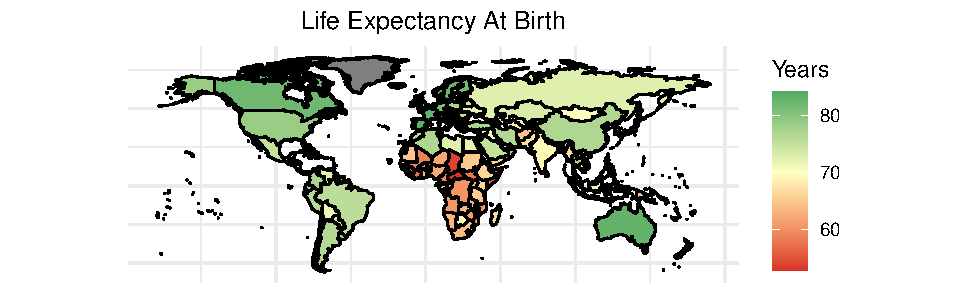
\includegraphics{final_report_files/figure-latex/unnamed-chunk-4-1} \end{center}

As we can observe from the plot, African countries tend to have a lower
life expectancy.

\hypertarget{alcohol-consumption-data}{%
\subsubsection{Alcohol Consumption
Data}\label{alcohol-consumption-data}}

\begin{Shaded}
\begin{Highlighting}[]
\KeywordTok{inner_join}\NormalTok{(world_map_df, alcohol_df, }\DataTypeTok{by =} \StringTok{"Country.Code"}\NormalTok{) }\OperatorTok
\StringTok{  }\KeywordTok{ggplot}\NormalTok{() }\OperatorTok{+}\StringTok{ }
\StringTok{  }\KeywordTok{geom_polygon}\NormalTok{(}\KeywordTok{aes}\NormalTok{(}\DataTypeTok{x =}\NormalTok{ long, }\DataTypeTok{y =}\NormalTok{ lat, }\DataTypeTok{group =}\NormalTok{ group, }\DataTypeTok{fill =}\NormalTok{ alcohol_consum), }\DataTypeTok{color =} \StringTok{"black"}\NormalTok{) }\OperatorTok{+}
\StringTok{  }\KeywordTok{coord_quickmap}\NormalTok{(}\DataTypeTok{expand =} \OtherTok{TRUE}\NormalTok{, }\DataTypeTok{clip =} \StringTok{"on"}\NormalTok{) }\OperatorTok{+}\StringTok{ }
\StringTok{  }\KeywordTok{theme_minimal}\NormalTok{() }\OperatorTok{+}
\StringTok{  }\KeywordTok{scale_fill_gradient2}\NormalTok{(}\DataTypeTok{low =} \StringTok{"#d73027"}\NormalTok{, }\DataTypeTok{mid =} \StringTok{"#ffffbf"}\NormalTok{, }\DataTypeTok{high =} \StringTok{"#1a9850"}\NormalTok{, }\DataTypeTok{midpoint =} \DecValTok{7}\NormalTok{) }\OperatorTok{+}\StringTok{ }
\StringTok{  }\KeywordTok{theme}\NormalTok{(}
    \DataTypeTok{plot.title =} \KeywordTok{element_text}\NormalTok{(}\DataTypeTok{hjust =} \FloatTok{0.5}\NormalTok{, }\DataTypeTok{size =} \DecValTok{12}\NormalTok{),}
    \DataTypeTok{axis.text =} \KeywordTok{element_blank}\NormalTok{(),}
    \DataTypeTok{axis.title =} \KeywordTok{element_blank}\NormalTok{()) }\OperatorTok{+}
\StringTok{  }\KeywordTok{labs}\NormalTok{(}
    \DataTypeTok{title =} \StringTok{"Alcohol Consumption Per Capita"}\NormalTok{,}
    \DataTypeTok{fill =} \StringTok{"Liters"}
\NormalTok{    )}
\end{Highlighting}
\end{Shaded}

\begin{center}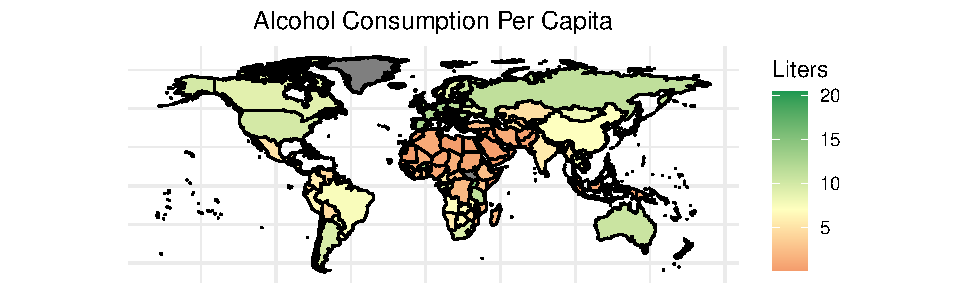
\includegraphics{final_report_files/figure-latex/unnamed-chunk-5-1} \end{center}

From the plot, we can observe that African countries tend to consume
less alcohol.

The two above visualizations would lead us to believe that there
\emph{is} a correlation between drinking more and living longer.
Formally, the independent variable in this study would be alcohol
consumption, and the dependent variable would be life expectancy.

Next, we would like to analyze GDP since we believe that to be the most
likely source of confounding bias in this relationship.

\hypertarget{gdp-data}{%
\subsubsection{GDP Data}\label{gdp-data}}

\begin{Shaded}
\begin{Highlighting}[]
\KeywordTok{inner_join}\NormalTok{(world_map_df, gdp_df, }\DataTypeTok{by =} \StringTok{"Country.Code"}\NormalTok{) }\OperatorTok
\StringTok{  }\KeywordTok{ggplot}\NormalTok{() }\OperatorTok{+}\StringTok{ }
\StringTok{  }\KeywordTok{geom_polygon}\NormalTok{(}\KeywordTok{aes}\NormalTok{(}\DataTypeTok{x =}\NormalTok{ long, }\DataTypeTok{y =}\NormalTok{ lat, }\DataTypeTok{group =}\NormalTok{ group, }\DataTypeTok{fill =}\NormalTok{ GDP), }\DataTypeTok{color =} \StringTok{"black"}\NormalTok{) }\OperatorTok{+}
\StringTok{  }\KeywordTok{coord_quickmap}\NormalTok{(}\DataTypeTok{expand =} \OtherTok{TRUE}\NormalTok{, }\DataTypeTok{clip =} \StringTok{"on"}\NormalTok{) }\OperatorTok{+}\StringTok{ }
\StringTok{  }\KeywordTok{theme_minimal}\NormalTok{() }\OperatorTok{+}
\StringTok{  }\KeywordTok{scale_fill_gradient2}\NormalTok{(}\DataTypeTok{low =} \StringTok{"white"}\NormalTok{, }\DataTypeTok{mid =} \StringTok{"white"}\NormalTok{, }\DataTypeTok{high =} \StringTok{"#1a9850"}\NormalTok{, }\DataTypeTok{midpoint =} \DecValTok{5000}\NormalTok{) }\OperatorTok{+}\StringTok{ }
\StringTok{  }\KeywordTok{theme}\NormalTok{(}
    \DataTypeTok{plot.title =} \KeywordTok{element_text}\NormalTok{(}\DataTypeTok{hjust =} \FloatTok{0.5}\NormalTok{, }\DataTypeTok{size =} \DecValTok{12}\NormalTok{),}
    \DataTypeTok{axis.text =} \KeywordTok{element_blank}\NormalTok{(),}
    \DataTypeTok{axis.title =} \KeywordTok{element_blank}\NormalTok{()) }\OperatorTok{+}
\StringTok{  }\KeywordTok{labs}\NormalTok{(}
    \DataTypeTok{title =} \StringTok{"GDP Per Capita"}\NormalTok{,}
    \DataTypeTok{fill =} \StringTok{"Dollars"}
\NormalTok{    )}
\end{Highlighting}
\end{Shaded}

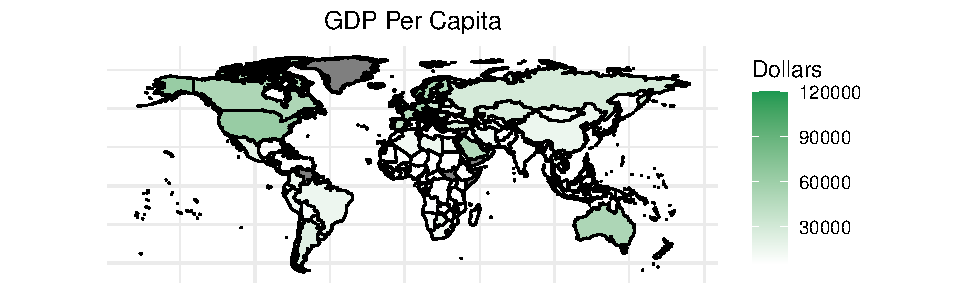
\includegraphics{final_report_files/figure-latex/unnamed-chunk-6-1.pdf}

Noticeably, the color of Africa is quite different from the rest of the
continents in all 3 maps shown. It is logical to assume that GDP might
be a confounding bias that the previous 2 maps fail to illustrate due to
its relationship with both of the independent (alcohol consumption) and
dependent (life expectancy) variables.

\begin{center}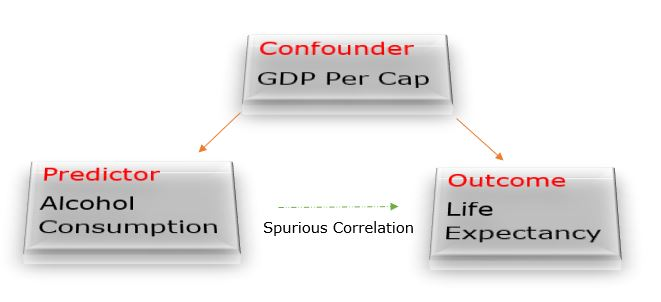
\includegraphics{pic/my_confounder} \end{center}

Now we will seek to illustrate that GDP has an impact on life expectancy
and alcohol consumption level.

\hypertarget{gdp-vs.-life-expectancy}{%
\subsubsection{GDP vs.~Life Expectancy}\label{gdp-vs.-life-expectancy}}

\begin{Shaded}
\begin{Highlighting}[]
\NormalTok{gdp_life_join <-}\StringTok{ }\KeywordTok{inner_join}\NormalTok{(gdp_df, life_exp_df, }\DataTypeTok{by =} \StringTok{"Country.Code"}\NormalTok{)}

\NormalTok{gdp_life_join }\OperatorTok\StringTok{ }
\StringTok{  }\KeywordTok{ggplot}\NormalTok{(}\KeywordTok{aes}\NormalTok{(GDP, life_exp)) }\OperatorTok{+}\StringTok{ }
\StringTok{  }\KeywordTok{geom_point}\NormalTok{() }\OperatorTok{+}\StringTok{ }
\StringTok{  }\KeywordTok{theme_classic}\NormalTok{() }\OperatorTok{+}
\StringTok{  }\KeywordTok{theme}\NormalTok{(}\DataTypeTok{plot.title =} \KeywordTok{element_text}\NormalTok{(}\DataTypeTok{hjust =} \FloatTok{0.5}\NormalTok{)) }\OperatorTok{+}
\StringTok{  }\KeywordTok{labs}\NormalTok{(}\DataTypeTok{x =} \StringTok{"GDP Per Capita in Log Scale (Dollars)"}\NormalTok{,}
       \DataTypeTok{y =} \StringTok{"Life Expectancy Per Capita (Years)"}\NormalTok{, }
       \DataTypeTok{title =} \StringTok{"GDP & Life Expectancy"}\NormalTok{) }\OperatorTok{+}\StringTok{ }
\StringTok{  }\KeywordTok{scale_x_continuous}\NormalTok{(}\DataTypeTok{trans =} \KeywordTok{log_trans}\NormalTok{(), }
                      \DataTypeTok{breaks =} \KeywordTok{trans_breaks}\NormalTok{(}\StringTok{"log"}\NormalTok{, }\ControlFlowTok{function}\NormalTok{(x) }\KeywordTok{exp}\NormalTok{(x)),}
                      \DataTypeTok{labels =} \KeywordTok{trans_format}\NormalTok{(}\StringTok{"log"}\NormalTok{, }\KeywordTok{math_format}\NormalTok{(e}\OperatorTok{^}\NormalTok{.x))) }\OperatorTok{+}
\StringTok{  }\KeywordTok{geom_smooth}\NormalTok{(}\DataTypeTok{se=}\NormalTok{F)}
\end{Highlighting}
\end{Shaded}

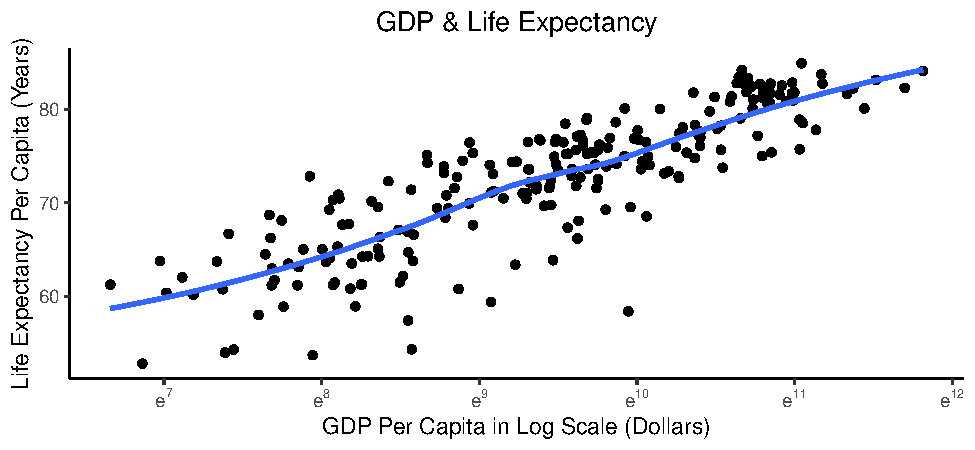
\includegraphics{final_report_files/figure-latex/unnamed-chunk-8-1.pdf}

To illustrate the model, let
\[life.exp = \beta_{0}+\beta_{1} * ln(gdp)\] When we increase GDP per
cap by 1\%, the new GDP, \(gdp_*\), becomes (1.01 * gdp).
\[life.exp_* = \beta_{0}+\beta_{1}  ln(gdp_*) = \beta_{0}+\beta_{1}  ln(1.01gdp)\]
\[= \beta_{0} +  \beta_{1}ln(gdp) + \beta_{1}ln(1.01)\]
\[= gdp + \beta_{1}  ln(1.01)\] \(\therefore\) one percent increase in
GDP is associated with a life expectancy increase of
\(\beta_{1} * ln(1.01)\) years.

\begin{Shaded}
\begin{Highlighting}[]
\NormalTok{mod1 <-}\StringTok{ }\KeywordTok{lm}\NormalTok{(life_exp }\OperatorTok{~}\StringTok{ }\KeywordTok{log}\NormalTok{(GDP), gdp_life_join)}
\KeywordTok{kable}\NormalTok{(}\KeywordTok{tidy}\NormalTok{(mod1), }\DataTypeTok{caption =} \StringTok{"Life Expectancy ~ ln(GDP)"}\NormalTok{)}
\end{Highlighting}
\end{Shaded}

\begin{longtable}[]{@{}lrrrr@{}}
\caption{Life Expectancy \textasciitilde{} ln(GDP)}\tabularnewline
\toprule
term & estimate & std.error & statistic & p.value\tabularnewline
\midrule
\endfirsthead
\toprule
term & estimate & std.error & statistic & p.value\tabularnewline
\midrule
\endhead
(Intercept) & 20.54514 & 2.1402435 & 9.599438 & 0\tabularnewline
log(GDP) & 5.50108 & 0.2255549 & 24.389094 & 0\tabularnewline
\bottomrule
\end{longtable}

We have obtained a P-value of less than 0.05 and a t-statistics of 24.4.
The result suggests that GDP has a statistically significant positive
relationship with life expectancy. That is, for one percent increase in
GDP is associated with a life expectancy increase of
\[5.5 * ln(1.1) \approx 0.5 \space years\]

\hypertarget{alcohol-consumption-vs.-gdp}{%
\subsubsection{Alcohol Consumption
vs.~GDP}\label{alcohol-consumption-vs.-gdp}}

\begin{Shaded}
\begin{Highlighting}[]
\KeywordTok{read.csv}\NormalTok{(}\StringTok{"data/geo_world.csv"}\NormalTok{) }\OperatorTok\StringTok{ }
\StringTok{  }\KeywordTok{select}\NormalTok{(Continent_Name, Three_Letter_Country_Code, Country_Name) }\OperatorTok\StringTok{ }
\StringTok{  }\KeywordTok{rename}\NormalTok{(}\DataTypeTok{Country.Code =}\NormalTok{ Three_Letter_Country_Code) }\OperatorTok\StringTok{ }
\StringTok{  }\KeywordTok{inner_join}\NormalTok{(alcohol_df, }\DataTypeTok{by =} \StringTok{"Country.Code"}\NormalTok{) }\OperatorTok\StringTok{ }
\StringTok{  }\KeywordTok{inner_join}\NormalTok{(gdp_df, }\DataTypeTok{by =} \StringTok{"Country.Code"}\NormalTok{) }\OperatorTok\StringTok{ }
\StringTok{  }\KeywordTok{ggplot}\NormalTok{(}\KeywordTok{aes}\NormalTok{(}\DataTypeTok{x =}\NormalTok{ alcohol_consum, }\DataTypeTok{y =}\NormalTok{ GDP, }\DataTypeTok{color =}\NormalTok{ Continent_Name)) }\OperatorTok{+}\StringTok{ }
\StringTok{  }\KeywordTok{geom_point}\NormalTok{() }\OperatorTok{+}
\StringTok{  }\KeywordTok{theme_minimal}\NormalTok{() }\OperatorTok{+}
\StringTok{  }\KeywordTok{theme}\NormalTok{(}\DataTypeTok{plot.title =} \KeywordTok{element_text}\NormalTok{(}\DataTypeTok{hjust =} \FloatTok{0.5}\NormalTok{)) }\OperatorTok{+}
\StringTok{  }\KeywordTok{labs}\NormalTok{(}\DataTypeTok{x =} \StringTok{"Alcohol Consumption Per Capita (Liters)"}\NormalTok{,}
       \DataTypeTok{y =} \StringTok{"GDP Per Capita (Dollars)"}\NormalTok{, }
       \DataTypeTok{title =} \StringTok{"Alcohol Consumption vs. GDP"}\NormalTok{,}
       \DataTypeTok{color =} \StringTok{"Continent"}\NormalTok{)}
\end{Highlighting}
\end{Shaded}

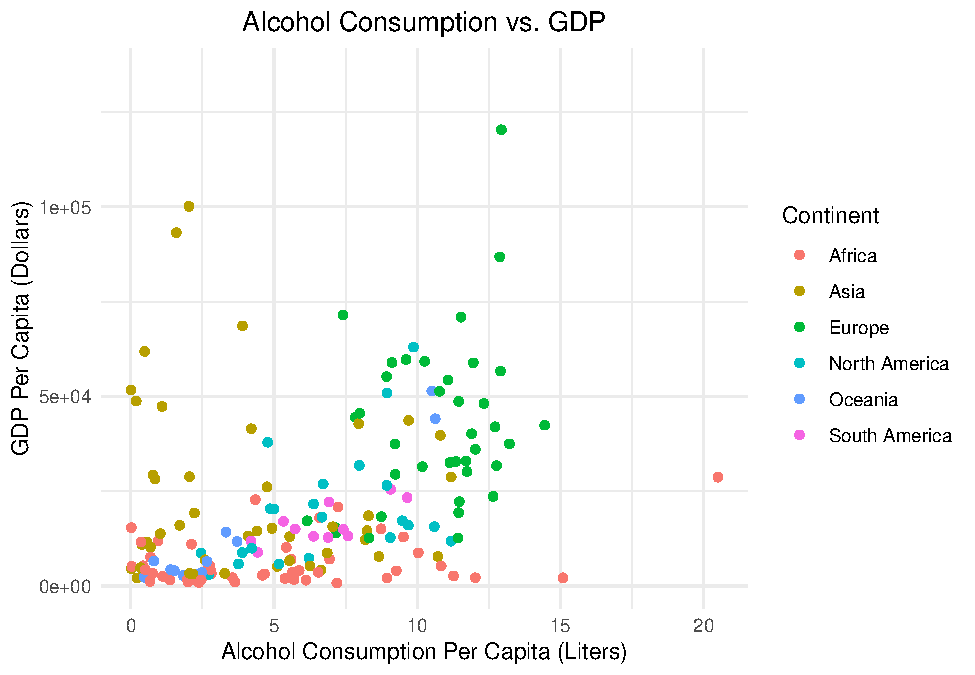
\includegraphics{final_report_files/figure-latex/unnamed-chunk-10-1.pdf}

Notice that European countries tend to have a higher GDP, and the
alcohol consumption level is also higher on average for European
countries. To further illustrate the point, we can plot alcohol
consumption vs life expectancy by continents.

\begin{Shaded}
\begin{Highlighting}[]
\KeywordTok{read.csv}\NormalTok{(}\StringTok{"data/geo_world.csv"}\NormalTok{) }\OperatorTok\StringTok{ }
\StringTok{  }\KeywordTok{select}\NormalTok{(Continent_Name, Three_Letter_Country_Code, Country_Name) }\OperatorTok\StringTok{ }
\StringTok{  }\KeywordTok{rename}\NormalTok{(}\DataTypeTok{Country.Code =}\NormalTok{ Three_Letter_Country_Code) }\OperatorTok\StringTok{ }
\StringTok{  }\KeywordTok{inner_join}\NormalTok{(alcohol_df, }\DataTypeTok{by =} \StringTok{"Country.Code"}\NormalTok{) }\OperatorTok\StringTok{ }
\StringTok{  }\KeywordTok{inner_join}\NormalTok{(life_exp_df, }\DataTypeTok{by =} \StringTok{"Country.Code"}\NormalTok{) }\OperatorTok\StringTok{ }
\StringTok{  }\KeywordTok{ggplot}\NormalTok{(}\KeywordTok{aes}\NormalTok{(alcohol_consum, life_exp, }\DataTypeTok{color =}\NormalTok{ Continent_Name)) }\OperatorTok{+}\StringTok{ }
\StringTok{  }\KeywordTok{geom_point}\NormalTok{() }\OperatorTok{+}\StringTok{ }
\StringTok{  }\KeywordTok{theme_minimal}\NormalTok{() }\OperatorTok{+}
\StringTok{  }\KeywordTok{theme}\NormalTok{(}\DataTypeTok{plot.title =} \KeywordTok{element_text}\NormalTok{(}\DataTypeTok{hjust =} \FloatTok{0.5}\NormalTok{)) }\OperatorTok{+}
\StringTok{  }\KeywordTok{facet_wrap}\NormalTok{(}\OperatorTok{~}\NormalTok{Continent_Name) }\OperatorTok{+}\StringTok{ }
\StringTok{  }\KeywordTok{stat_smooth}\NormalTok{(}\DataTypeTok{method =} \StringTok{"lm"}\NormalTok{) }\OperatorTok{+}
\StringTok{  }\KeywordTok{labs}\NormalTok{(}
    \DataTypeTok{x =} \StringTok{"Alcohol Consumption Per Capita (Liters)"}\NormalTok{,}
    \DataTypeTok{y =} \StringTok{"Life Expectancy Per Capita (Years)"}\NormalTok{,}
    \DataTypeTok{title =} \StringTok{"Alcohol Consumption vs. Life Expectancy by Continent"}
\NormalTok{  )}
\end{Highlighting}
\end{Shaded}

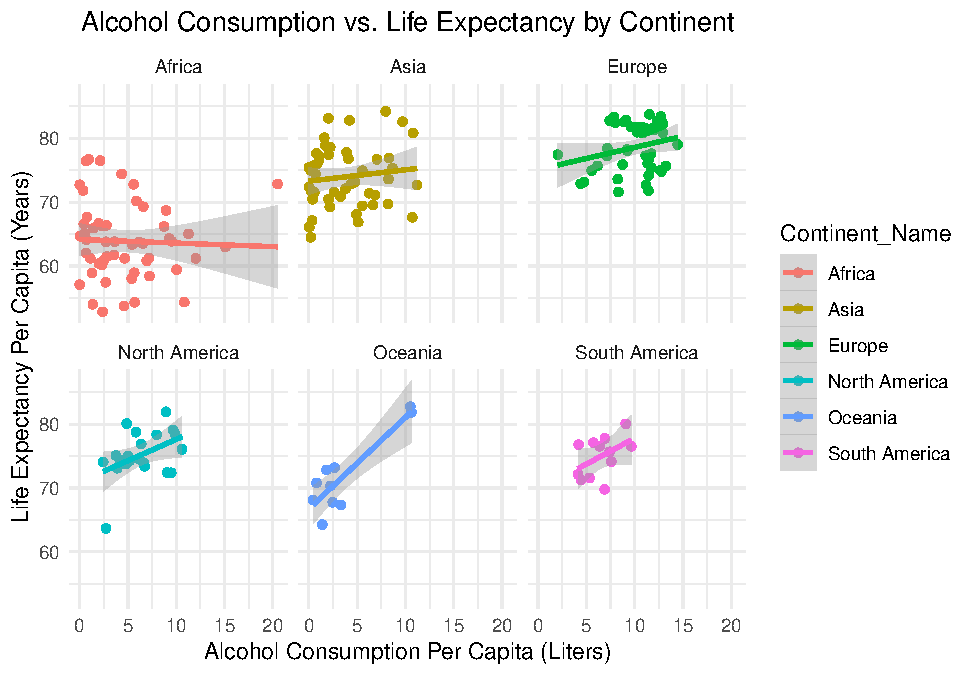
\includegraphics{final_report_files/figure-latex/unnamed-chunk-11-1.pdf}

Notice that there is not a strong positive correlation between alcohol
consumption and life expectancy for African countries. That is to say,
the life expectancy of African people would not get higher by drinking
more alcohol.

To directly evaluate the relationship between alcohol consumption and
life expectancy, we will take all countries into consideration and
cluster the data with a k-means method.

\hypertarget{k-means-training-data}{%
\subsubsection{K-Means (Training Data)}\label{k-means-training-data}}

\begin{Shaded}
\begin{Highlighting}[]
\NormalTok{alcohol_life_df <-}\StringTok{ }\KeywordTok{inner_join}\NormalTok{(alcohol_df, life_exp_df) }
\NormalTok{filter_alcohol_life_df <-}\StringTok{ }\NormalTok{alcohol_life_df }\OperatorTok\StringTok{ }
\StringTok{  }\KeywordTok{select}\NormalTok{(alcohol_consum, life_exp) }\OperatorTok\StringTok{ }
\StringTok{  }\KeywordTok{filter}\NormalTok{(}\OperatorTok{!}\KeywordTok{is.na}\NormalTok{(alcohol_consum), }\OperatorTok{!}\KeywordTok{is.na}\NormalTok{(life_exp))}

\NormalTok{k_2means <-}\StringTok{ }\KeywordTok{kmeans}\NormalTok{(filter_alcohol_life_df, }\DataTypeTok{centers =} \DecValTok{3}\NormalTok{)}

\KeywordTok{plot}\NormalTok{(filter_alcohol_life_df[k_2means}\OperatorTok{$}\NormalTok{cluster }\OperatorTok{==}\StringTok{ }\DecValTok{1}\NormalTok{, ], }\DataTypeTok{col =} \StringTok{"blue"}\NormalTok{, }\DataTypeTok{ylim=}\KeywordTok{c}\NormalTok{(}\DecValTok{50}\NormalTok{,}\DecValTok{90}\NormalTok{), }
     \DataTypeTok{main =} \StringTok{"Training Dataset with K = 3"}\NormalTok{, }\DataTypeTok{xlab =} \StringTok{"Alcohol Consumption Per Capita (Liters)"}\NormalTok{,}
     \DataTypeTok{ylab =} \StringTok{"Life Expectancy Per Capita (Years)"}\NormalTok{)}
\KeywordTok{points}\NormalTok{(filter_alcohol_life_df[k_2means}\OperatorTok{$}\NormalTok{cluster }\OperatorTok{==}\StringTok{ }\DecValTok{2}\NormalTok{, ], }\DataTypeTok{col =} \StringTok{"red"}\NormalTok{)}
\KeywordTok{points}\NormalTok{(filter_alcohol_life_df[k_2means}\OperatorTok{$}\NormalTok{cluster }\OperatorTok{==}\StringTok{ }\DecValTok{3}\NormalTok{, ], }\DataTypeTok{col =} \StringTok{"green"}\NormalTok{)}
\end{Highlighting}
\end{Shaded}

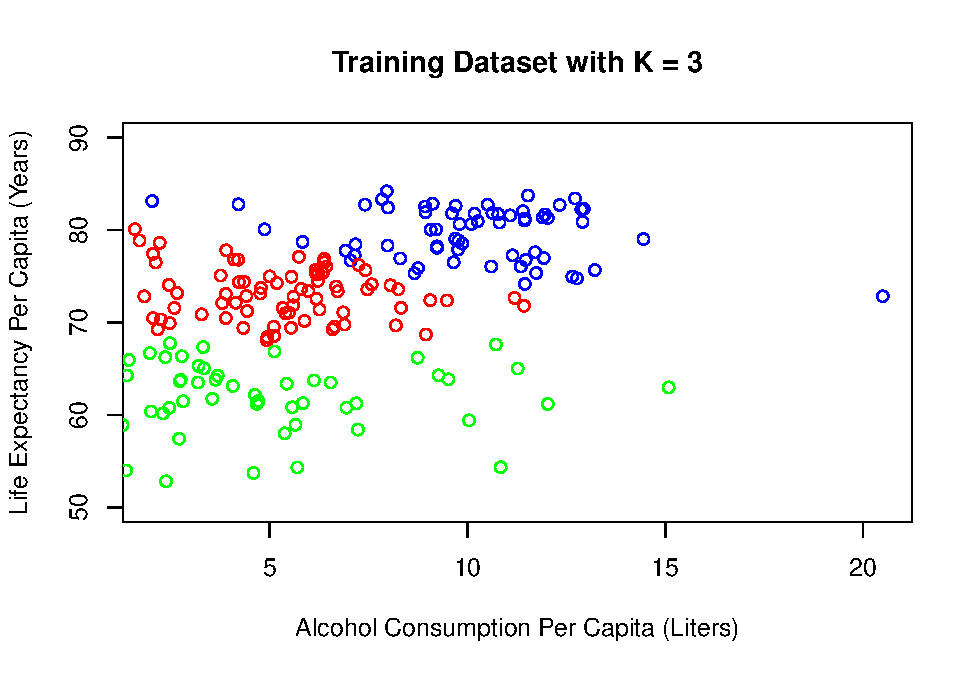
\includegraphics{final_report_files/figure-latex/unnamed-chunk-12-1.pdf}
The findings from K-means clustering are not particularly useful in this
case because we know the labels of the data. We can infer that the top
right region corresponds to European countries, while the bottom region
correspond to African countries.

\hypertarget{labeled-data}{%
\subsubsection{Labeled data}\label{labeled-data}}

\begin{Shaded}
\begin{Highlighting}[]
\KeywordTok{read.csv}\NormalTok{(}\StringTok{"data/geo_world.csv"}\NormalTok{) }\OperatorTok\StringTok{ }
\StringTok{  }\KeywordTok{select}\NormalTok{(Continent_Name, Three_Letter_Country_Code, Country_Name) }\OperatorTok\StringTok{ }
\StringTok{  }\KeywordTok{rename}\NormalTok{(}\DataTypeTok{Country.Code =}\NormalTok{ Three_Letter_Country_Code) }\OperatorTok\StringTok{ }
\StringTok{  }\KeywordTok{inner_join}\NormalTok{(alcohol_df, }\DataTypeTok{by =} \StringTok{"Country.Code"}\NormalTok{) }\OperatorTok\StringTok{ }
\StringTok{  }\KeywordTok{inner_join}\NormalTok{(life_exp_df, }\DataTypeTok{by =} \StringTok{"Country.Code"}\NormalTok{) }\OperatorTok\StringTok{ }
\StringTok{  }\KeywordTok{ggplot}\NormalTok{(}\KeywordTok{aes}\NormalTok{(}\DataTypeTok{x =}\NormalTok{ alcohol_consum, }\DataTypeTok{y =}\NormalTok{ life_exp,}
             \DataTypeTok{color =}\NormalTok{ Continent_Name)) }\OperatorTok{+}\StringTok{ }
\StringTok{  }\KeywordTok{geom_point}\NormalTok{() }\OperatorTok{+}
\StringTok{  }\KeywordTok{xlim}\NormalTok{(}\KeywordTok{c}\NormalTok{(}\DecValTok{0}\NormalTok{,}\DecValTok{17}\NormalTok{)) }\OperatorTok{+}\StringTok{ }
\StringTok{  }\KeywordTok{theme_minimal}\NormalTok{() }\OperatorTok{+}
\StringTok{  }\KeywordTok{theme}\NormalTok{(}\DataTypeTok{plot.title =} \KeywordTok{element_text}\NormalTok{(}\DataTypeTok{hjust =} \FloatTok{0.5}\NormalTok{)) }\OperatorTok{+}
\StringTok{  }\KeywordTok{labs}\NormalTok{(}
    \DataTypeTok{x =} \StringTok{"Alcohol Consumption Per Capita (Liters)"}\NormalTok{,}
    \DataTypeTok{y =} \StringTok{"Life Expectancy Per Capita (Years)"}\NormalTok{,}
    \DataTypeTok{title =} \StringTok{"Alcohol Consumption vs. Life Expectancy by Continent"}\NormalTok{,}
    \DataTypeTok{color =} \StringTok{"Continent"}
\NormalTok{  )}
\end{Highlighting}
\end{Shaded}

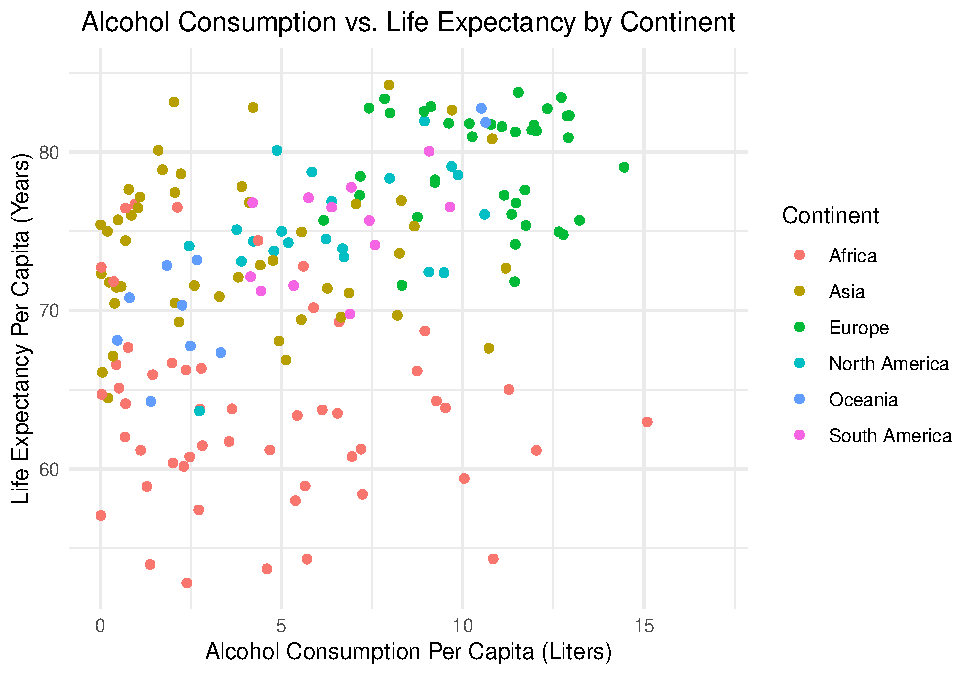
\includegraphics{final_report_files/figure-latex/unnamed-chunk-13-1.pdf}

Again, we can clearly see that European countries tend to cluster around
the top right corner, meaning that European countries have a higher life
expectancy, and they tend to consume more alcohol as well. However,
there is no evidence indicating that there is a causal relationship
between alcohol consumption and life expectancy based on plotting the
two variables directly as shown below.

\begin{center}\rule{0.5\linewidth}{0.5pt}\end{center}

\hypertarget{results}{%
\subsection{Results}\label{results}}

\begin{Shaded}
\begin{Highlighting}[]
\NormalTok{alcohol_life_df }\OperatorTok\StringTok{ }
\StringTok{  }\KeywordTok{ggplot}\NormalTok{(}\KeywordTok{aes}\NormalTok{(}\DataTypeTok{x =}\NormalTok{ alcohol_consum, }\DataTypeTok{y =}\NormalTok{ life_exp)) }\OperatorTok{+}\StringTok{ }
\StringTok{  }\KeywordTok{geom_point}\NormalTok{() }\OperatorTok{+}\StringTok{ }
\StringTok{  }\KeywordTok{theme_minimal}\NormalTok{() }\OperatorTok{+}
\StringTok{  }\KeywordTok{theme}\NormalTok{(}\DataTypeTok{plot.title =} \KeywordTok{element_text}\NormalTok{(}\DataTypeTok{hjust =} \FloatTok{0.5}\NormalTok{)) }\OperatorTok{+}
\StringTok{  }\KeywordTok{labs}\NormalTok{(}
    \DataTypeTok{title =} \StringTok{"Alcohol Consumption vs. Life Expectancy"}\NormalTok{,}
    \DataTypeTok{x =} \StringTok{"Alcohol Consumption Per Capita (Liters)"}\NormalTok{,}
    \DataTypeTok{y =} \StringTok{"Life Expectancy Per Capita (Years)"}\NormalTok{)}
\end{Highlighting}
\end{Shaded}

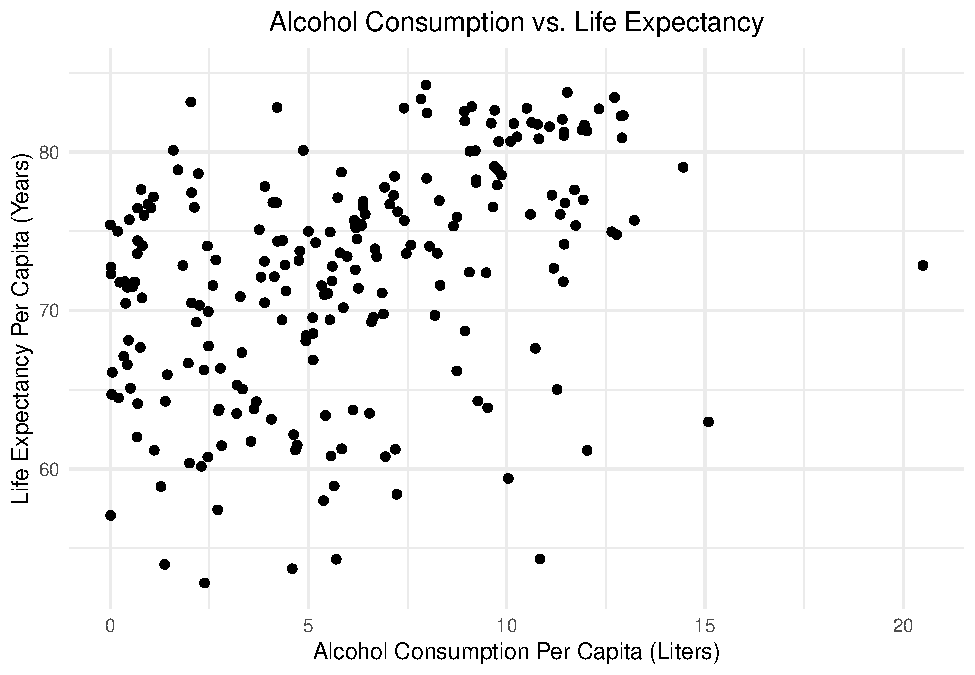
\includegraphics{final_report_files/figure-latex/unnamed-chunk-14-1.pdf}

The above scatterplot shows no obvious correlation or pattern in the
data, and we will explore that relationship mathematically with a linear
regression model below:

\begin{Shaded}
\begin{Highlighting}[]
\NormalTok{merge_al_life_gdp <-}\StringTok{ }\NormalTok{alcohol_life_df }\OperatorTok\StringTok{ }
\StringTok{  }\KeywordTok{inner_join}\NormalTok{(gdp_df, }\DataTypeTok{by =} \StringTok{"Country.Code"}\NormalTok{) }\OperatorTok\StringTok{ }
\StringTok{  }\KeywordTok{select}\NormalTok{(alcohol_consum, life_exp, GDP) }\OperatorTok\StringTok{ }
\StringTok{  }\KeywordTok{filter}\NormalTok{(}\OperatorTok{!}\KeywordTok{is.na}\NormalTok{(alcohol_consum), }\OperatorTok{!}\KeywordTok{is.na}\NormalTok{(life_exp), }\OperatorTok{!}\KeywordTok{is.na}\NormalTok{(GDP))}


\NormalTok{model <-}\StringTok{ }\KeywordTok{lm}\NormalTok{(merge_al_life_gdp, }\DataTypeTok{formula =}\NormalTok{ life_exp }\OperatorTok{~}\StringTok{ }\NormalTok{alcohol_consum }\OperatorTok{+}\StringTok{ }
\StringTok{              }\NormalTok{GDP }\OperatorTok{+}\StringTok{ }\NormalTok{alcohol_consum}\OperatorTok{:}\NormalTok{GDP)}

\KeywordTok{kable}\NormalTok{(}\KeywordTok{tidy}\NormalTok{(model), }\DataTypeTok{caption =} \StringTok{"Life Expectancy ~ Alcohol Consumption + GDP"}\NormalTok{)}
\end{Highlighting}
\end{Shaded}

\begin{longtable}[]{@{}lrrrr@{}}
\caption{Life Expectancy \textasciitilde{} Alcohol Consumption +
GDP}\tabularnewline
\toprule
term & estimate & std.error & statistic & p.value\tabularnewline
\midrule
\endfirsthead
\toprule
term & estimate & std.error & statistic & p.value\tabularnewline
\midrule
\endhead
(Intercept) & 66.1936295 & 0.8189934 & 80.8231570 &
0.0000000\tabularnewline
alcohol\_consum & 0.1830770 & 0.1354016 & 1.3521033 &
0.1777498\tabularnewline
GDP & 0.0002516 & 0.0000329 & 7.6572802 & 0.0000000\tabularnewline
alcohol\_consum:GDP & -0.0000015 & 0.0000039 & -0.3822081 &
0.7026810\tabularnewline
\bottomrule
\end{longtable}

Interpretation regarding predictor \texttt{alcohol\_consum}:

\textbf{estimate}: This column is used to predict the value of the
response variable. In this case, we can conclude that, while holding all
other predictor variables constant, the change in life expectancy
associated with a Liter increase of alcohol consumption is 0.18 years.
(However, this number alone is meaningless if we don't take confidence
interval and p value into consideration)

\textbf{std.error}: The average amount that the estimate deviates from
the actual value. This number is often used to calculate the confidence
interval. We see that a std.error is 0.14 which is relative large to the
coefficient estimate obtained.

\textbf{statistics}: This is the equivalent of the t-value, which is
calculated using estimate / std.error. If the t-value is relatively
high, the coefficient is statistically significant. As we can see here,
the t-value for \texttt{alcohol\ consumption} is a lot lower than the
t-value for \texttt{GDP}.

\textbf{p.value}: This is the p-value for the t test. The smaller the
P-value, the stronger the statistical significance. In other words, it
is very likely that the relationship between the dependent variable and
independent variable is due to random chance. Due to the large P-value
(\textgreater0.05), we can't reject the null hypothesis that there is no
relationship between alcohol consumption and life expectancy. In other
words, ``there is no relationship between alcohol consumption and life
expectancy'' still holds true.

\hypertarget{confounding-bias-and-conclusion}{%
\subsection{Confounding Bias and
Conclusion}\label{confounding-bias-and-conclusion}}

As can be seen in the above linear model results, our p-value result for
alcohol consumption's correlation with life expectancy is greater than
0.05, leading us to fail to reject the null hypothesis and conclude that
there is no relationship based upon the data within this report. We
included GDP in the linear model due to the clear relationship and
possible confounding that we had uncovered throughout the report. There
very well may be other confounding factors that are not present in our
data set such as cultural norms (smoking and drinking together,
early-age drinking laws, etc.), types of alcoholic beverages that are
being consumed (do wine, beer, or hard alcohol drinks change the
relationship?), domestic instability (do war-torn countries drink
more/less and have lower life-expectancy? do peaceful countries drink
more/less and live longer?), and other factors that may be harder to
quantify. We again have to acknowledge the limitations of the data set
itself and the simple regression model that's been leveraged. The data
sets are limited by the accuracy of the data collection techniques of
the countries themselves and since the estimations are on such a large
scale the errors could have massive implications on our regression
models and data analysis. These statistics could be used to forge new
policies and write new laws so there could also be some reason for
countries to misreport or inaccurately record numbers such as these.

Even with all of these limitations and possible confounders in play, the
relationship was clearly far from a strong correlation (as seen in the
many plots) so we are quite confident in our conclusion that there is no
direct relationship between alcohol consumption and life expectancy
based on the World Bank data alone.

\begin{center}\rule{0.5\linewidth}{0.5pt}\end{center}

Future Research: It seems like there is a strong correlation between GDP
per cap and life expectancy. Can we say that the higher the GDP, the
higher the life expectancy? Or does the pattern only exist to a certain
degree? Based on the GDP vs.~life expectancy plot, it makes sense that
the slope decreases gradually as GDP approaches a certain number due to
the fact that humans can't live forever. However, could it be that rich
countries tend to exhibit unhealthy habits such as smoking and fast
food, such that it lowers their life expectancy? \newpage

An excellent way to visualize the three entities is to use a 3D plot. I
tried to visualize the regression line in 3D (the 2D regression becomes
a plane). Based on the live 3D plot, we can clearly see that there is a
strong correlation between GDP and life expectancy. We don't observe a
strong positive or negative relationship between alcohol consumption and
life expectancy. That being said, we can't see the benefits of the 3D
plot because R Markdown doesn't render live plots that we can drag
around.

\end{document}
